\iffalse
\let\negmedspace\undefined
\let\negthickspace\undefined
\documentclass[journal,12pt,twocolumn]{IEEEtran}
\usepackage{cite}
\usepackage{amsmath,amssymb,amsfonts,amsthm}
\usepackage{algorithmic}
\usepackage{graphicx}
\usepackage{textcomp}
\usepackage{xcolor}
\usepackage{txfonts}
\usepackage{listings}
\usepackage{enumitem}
\usepackage{mathtools}
\usepackage{gensymb}
\usepackage{comment}
\usepackage[breaklinks=true]{hyperref}
\usepackage{tkz-euclide} 
\usepackage{listings}
\usepackage{gvv}                                        
\def\inputGnumericTable{}                                 
\usepackage[latin1]{inputenc}                                
\usepackage{color}                                            
\usepackage{array}                                            
\usepackage{longtable}                                       
\usepackage{calc}                                             
\usepackage{multirow}                                         
\usepackage{hhline}                                           
\usepackage{ifthen}                                           
\usepackage{lscape}
\newtheorem{theorem}{Theorem}[section]
\newtheorem{problem}{Problem}
\newtheorem{proposition}{Proposition}[section]
\newtheorem{lemma}{Lemma}[section]
\newtheorem{corollary}[theorem]{Corollary}
\newtheorem{example}{Example}[section]
\newtheorem{definition}[problem]{Definition}
\newcommand{\BEQA}{\begin{eqnarray}}
\newcommand{\EEQA}{\end{eqnarray}}
\newcommand{\define}{\stackrel{\triangle}{=}}
\theoremstyle{remark}
\newtheorem{rem}{Remark}
\begin{document}

\bibliographystyle{IEEEtran}
\vspace{3cm}

\title{GATE: IN - 50.2023}
\author{EE23BTECH11224 - Sri Krishna Prabhas Yadla$^{*}$% <-this % stops a space
}
\maketitle
\newpage
\bigskip

\renewcommand{\thefigure}{\arabic{figure}}
\renewcommand{\thetable}{\arabic{table}}


\vspace{3cm}
\textbf{Question:} The phase margin of the transfer function $G(s) = \frac{2(1-s)}{(1+s)^2}$ is \rule{1cm}{0.15mm} degrees. (rounded off to the nearest integer). \hfill (GATE IN 2023)\\
\solution
\fi
\begin{table}[htbp]
	\centering
	\def\arraystrech{1.5}
	\begin{tabular}{|c|c|}
\hline
\textbf{Parameters} & \textbf{Description} \\
\hline
$\omega_c$ & crossover frequency \\
\hline
$\angle G(j\omega)$ & phase angle of the transfer function \\
\hline
$PM$ & $\angle G(j\omega_c)+180\degree$; Phase Margin\\
\hline
\end{tabular}

	\caption{Parameters}
	\label{tab:parameters}
\end{table}
\newline
Considering $s=j\omega$,
\begin{align}
	G(j\omega) &= \frac{2(1-j\omega)}{(1+j\omega)^2} \\
	&= \frac{2(1-j\omega)^3}{\abs{1+j\omega}^4}\\
	&= \frac{2}{(1+\omega^2)^2}(1-j\omega)^3 \\
	&= \frac{2}{\sqrt{1+\omega^2}}(e^{-j\omega})^3 \\
	\implies \abs{G(j\omega)} &= \frac{2}{\sqrt{1+\omega^2}} \\
	\implies \angle G(j\omega) &= 3\tan^{-1}(-\omega)
\end{align}
At $\omega = \omega_c$, $Gain = 0$
\begin{align}
	\implies \abs{G(j\omega_c)} &= 1 \\
	\frac{2}{\sqrt{1+\omega_c^2}} &= 1 \\
	\implies \omega_c &= \sqrt{3} \\
	\angle G(j\omega_c) &= 3\tan^{-1}(-\sqrt{3}) \\
	&= -180\degree
\end{align}
From \tabref{tab:parameters},
\begin{align}
	PM &= 0\degree
\end{align}
\begin{figure}[htbp]
	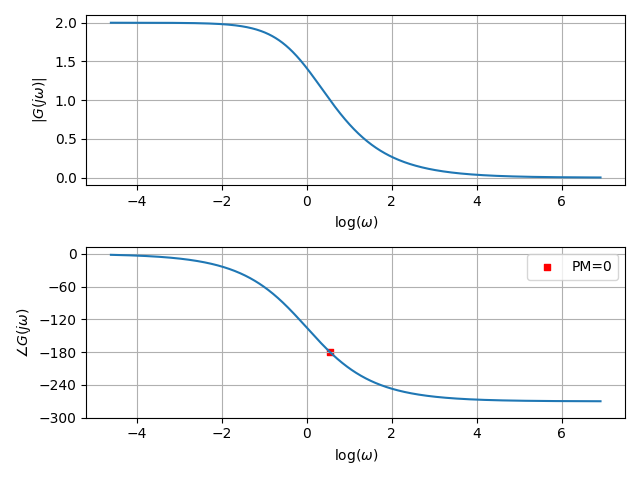
\includegraphics[width=\columnwidth]{2023/IN/50/figs/bode.png}
	\caption{Bode Plot of Transfer Function $G(s)$}
	\label{fig:bode}
\end{figure}
